% !TeX program = xelatex
\documentclass[11pt,a4paper]{article}

% -------------------------------------------------
% Packages
% -------------------------------------------------
\usepackage{kotex}
\usepackage{fontspec}
\usepackage{amsmath,amssymb,bm,mathtools}
\usepackage[left=24mm,right=24mm,top=23mm,bottom=25mm]{geometry}
\usepackage{booktabs,array}
\usepackage{enumitem}
\usepackage{setspace}
\usepackage{xcolor}
\usepackage{colortbl}
\usepackage{tikz}
\usepackage{pifont}
\usetikzlibrary{positioning,arrows.meta,calc,fit,decorations.pathreplacing}
\usepackage[most]{tcolorbox}
\usepackage{listings}
\usepackage{hyperref}
\usepackage{fancyhdr}

\setstretch{1.14}
\setlength{\parindent}{0pt}
\setlength{\parskip}{0.55em}

% -------------------------------------------------
% Colors and boxes
% -------------------------------------------------
\definecolor{deepblue}{RGB}{34,71,120}
\definecolor{softblue}{RGB}{239,246,253}
\definecolor{softgray}{RGB}{246,247,249}
\definecolor{softgreen}{RGB}{239,249,242}
\definecolor{softyellow}{RGB}{255,249,229}
\definecolor{codegray}{RGB}{248,248,248}

\newtcolorbox{keybox}[1][]{
  colback=softblue,
  colframe=deepblue,
  boxrule=0.7pt,
  arc=2mm,
  title=#1,
  fonttitle=\bfseries
}

\newtcolorbox{thinkbox}[1][]{
  colback=softyellow,
  colframe=orange!70!black,
  boxrule=0.6pt,
  arc=2mm,
  title=#1,
  fonttitle=\bfseries
}

\newtcolorbox{remarkbox}[1][]{
  colback=softgray,
  colframe=black!45,
  boxrule=0.5pt,
  arc=2mm,
  title=#1,
  fonttitle=\bfseries
}

\newtcolorbox{mlbox}[1][]{
  colback=softgreen,
  colframe=green!45!black,
  boxrule=0.6pt,
  arc=2mm,
  title=#1,
  fonttitle=\bfseries
}

% -------------------------------------------------
% Code style
% -------------------------------------------------
\lstdefinestyle{pythonstyle}{
  language=Python,
  backgroundcolor=\color{codegray},
  basicstyle=\ttfamily\small,
  keywordstyle=\bfseries,
  commentstyle=\itshape\color{black!60},
  stringstyle=\color{black!75},
  numbers=left,
  numberstyle=\tiny\color{black!55},
  numbersep=8pt,
  frame=single,
  rulecolor=\color{black!25},
  breaklines=true,
  showstringspaces=false,
  tabsize=4,
  columns=fullflexible,
  keepspaces=true
}
\lstset{style=pythonstyle}

% -------------------------------------------------
% Math commands
% -------------------------------------------------
\newcommand{\R}{\mathbb{R}}
\newcommand{\grad}{\nabla}
\newcommand{\vect}[1]{\bm{#1}}
\newcommand{\T}{^{\mathsf T}}
\newcommand{\loss}{\mathcal{L}}
\newcommand{\sigmoid}{\sigma}
\newcommand{\pd}[2]{\frac{\partial #1}{\partial #2}}
\newcommand{\softmax}{\operatorname{softmax}}

% -------------------------------------------------
% Header / footer
% -------------------------------------------------
\pagestyle{fancy}
\fancyhf{}
\lhead{Introduction to Deep Learning and Practice}
\rhead{Techniques for Training}
\cfoot{\thepage}
\renewcommand{\headrulewidth}{0.4pt}
\setlength{\headheight}{14pt}

\hypersetup{
  colorlinks=true,
  linkcolor=deepblue,
  urlcolor=deepblue
}

% =================================================
\begin{document}
\begin{center}
{\LARGE\bfseries 학습 관련 기술: 별도 심화 자료}\\[0.4em]
{\large 실제 딥러닝의 optimizer와 2차 미분을 쓰는 방법}\\[0.4em]
{\normalsize 학생용 강의안과 분리한 선택 읽기 자료}
\end{center}
\appendix

\section{부록: 실제 딥러닝의 optimizer와 2차 미분을 쓰는 방법}\label{app:opt}
% =================================================

본문에서는 SGD, 모멘텀, AdaGrad, RMSProp, Adam의 원리를 살펴보았다.
이 부록에서는 두 가지 질문을 다룬다.
\begin{enumerate}[label=(\arabic*)]
\item 요즘 실제 딥러닝에서는 어떤 optimizer가 쓰이는가?
\item ``Gradient Descent와 Newton's method'' 시간에 본 Newton 방법처럼
\textbf{2차 미분(곡률) 정보}를 쓰는 방법은 딥러닝에서 어떻게 되는가?
\end{enumerate}
이 부록에서는 매개변수 전체를 한 줄로 펼친 열벡터 $\theta\in\R^n$으로 쓰고,
$g_k=\nabla L(\theta_k)$, Hessian을 $H=\nabla^2L$로 쓴다.

\begin{remarkbox}[이 부록을 읽는 방법]
이 부록은 시험 범위가 아니라 \textbf{읽을거리}이다.
Armijo $\cdot$ Wolfe 조건, BFGS 갱신식, two-loop recursion 같은 세부 수식은
최적화 이론(수치최적화) 과목에서 자세히 다루는 내용이므로 지금 모두 이해하지 않아도 된다.
대신 다음 두 가지에 집중해서 읽자.
\begin{itemize}[leftmargin=1.5em]
\item 각 방법이 \textbf{무엇을 근사하려고 하는가} (대부분 Hessian, 즉 곡률 정보이다)
\item 그 방법이 딥러닝에서 \textbf{왜 잘 쓰이는가, 또는 왜 잘 쓰이지 않는가}
\end{itemize}
이번 주에 배운 SGD와 Adam 너머에 어떤 최적화 이론이 있고,
그것이 지금도 딥러닝 연구에 어떻게 적용되고 있는지 감을 잡는 것이 목표이다.
\end{remarkbox}

% -------------------------------------------------
\subsection{요즘 실제로 쓰이는 optimizer}
% -------------------------------------------------

본문의 기법들이 모두 같은 비중으로 쓰이는 것은 아니다.
대략적인 경향은 다음과 같다.

\begin{center}
\begin{tabular}{@{}lp{0.68\textwidth}@{}}
\toprule
optimizer & 주로 쓰이는 곳 \\
\midrule
\textbf{AdamW} & 사실상의 기본값. Transformer, 대규모 언어모델(LLM), 확산(diffusion) 모델 등 최신 모델 대부분 \\[3pt]
\textbf{SGD + 모멘텀} & 이미지 분류 CNN (ResNet 등). 잘 조정하면 일반화 성능이 Adam보다 좋은 경우가 많다.
Nesterov 모멘텀을 함께 쓰기도 한다. \\[3pt]
Adam & AdamW 이전의 표준. 작은 모델과 실습에서는 여전히 많이 쓰인다. \\[3pt]
RMSProp & 예전에 강화학습(DQN 등)과 RNN에서 많이 쓰였으나 비중이 줄었다. \\[3pt]
AdaGrad & 추천 시스템처럼 희소한(sparse) 특징이 많은 문제 정도에서 쓰인다. \\
\bottomrule
\end{tabular}
\end{center}

\paragraph{AdaGrad는 왜 배우는가?}
AdaGrad는 지금 거의 쓰이지 않지만, ``\textbf{매개변수마다 학습률을 다르게}''라는 아이디어의 출발점이다.
그 약점을 고친 것이 RMSProp이고, RMSProp에 모멘텀을 합친 것이 Adam이다.
즉 AdaGrad $\rightarrow$ RMSProp $\rightarrow$ Adam $\rightarrow$ AdamW로 이어지는 흐름을 이해하기 위해 배운다.

\paragraph{AdamW.}
Adam에 \textbf{weight decay(가중치 감소)}를 올바르게 붙인 방법이다 (Loshchilov \& Hutter, 2019).
Adam의 손실에 L2 정규화 항을 그냥 더하면 그 항의 gradient도 $\sqrt{\hat v}$로 나뉘어,
정규화의 세기가 매개변수마다 들쭉날쭉해진다.
AdamW는 감소 항을 갱신식에서 따로 떼어 적용한다.
갱신식과 코드는 학생용 강의안의 AdamW 절에서 살펴보았다.

\paragraph{최근에 연구되고 쓰이는 방법들.}
아직 AdamW만큼 표준은 아니지만 다음과 같은 방법들이 있다.
\begin{itemize}[leftmargin=1.8em]
\item \textbf{Lion} (2023): gradient의 \textbf{부호}만 사용해 갱신하여 메모리를 아낀다.
\item \textbf{Adafactor}: Adam의 2차 moment $v$를 행과 열의 통계로 압축해 메모리를 아낀다. 큰 언어모델 학습에 쓰였다.
\item \textbf{LAMB, LARS}: 층마다 갱신량의 크기를 조절하여 \textbf{아주 큰 미니배치}로 학습할 때 쓴다.
\item \textbf{Shampoo, Muon}: 가중치 행렬의 구조를 이용해 곡률을 근사하는 방법 (\ref{app:largescale}절).
\end{itemize}

\paragraph{optimizer보다 중요할 때가 많은 것: 학습률 스케줄.}
실무에서는 어떤 optimizer를 고르느냐보다 \textbf{학습률을 단계에 따라 어떻게 바꾸느냐}가
성능에 더 큰 영향을 주는 경우가 많다. 대표적인 것은
처음 $K_w$단계 동안 학습률을 $0$에서 서서히 올리는 \textbf{warmup}과,
그 뒤 남은 $K$단계 동안 학습률을 코사인 곡선을 따라 줄이는 \textbf{cosine 감소}이다.
\[
\alpha_k=
\begin{cases}
\alpha_{\max}\,\dfrac{k}{K_w}, & 0\le k<K_w\\[10pt]
\alpha_{\min}+\dfrac12\bigl(\alpha_{\max}-\alpha_{\min}\bigr)\Bigl(1+\cos\dfrac{\pi\,(k-K_w)}{K}\Bigr), & K_w\le k\le K_w+K
\end{cases}
\]
처음에는 아직 $m$, $v$ 같은 통계가 불안정하므로 작은 보폭으로 시작하고,
마지막에는 보폭을 줄여 최솟값 근처에서 흔들리지 않게 한다
(본문의 RMSProp 그림에서 최솟값 근처의 흔들림을 떠올려 보자).
weight decay의 세기와 함께 이 스케줄이 최종 성능을 크게 좌우한다.

% -------------------------------------------------
\subsection{SGD는 언제 수렴하는가?}\label{app:sgdconv}
% -------------------------------------------------

``Gradient Descent와 Newton's method'' 시간에는 정확한 gradient를 쓰는 경사하강법이
$|1-\alpha f''|<1$이면 수렴함을 보았고, 본문 학생용 강의안의 SGD 절에서도 같은 조건을 확인하였다.
그런데 실제 SGD는 \textbf{미니배치}로 gradient를 계산하므로 gradient에 \textbf{잡음}이 섞인다.
잡음이 있어도 수렴할까? 학습률은 어떻게 정해야 할까?

\paragraph{1. 가정: 잡음이 섞인 gradient.}
$k$번째 단계에서 실제로 쓰는 gradient를
\[
\hat g_k=\nabla L(\theta_k)+\xi_k
\]
라 하자. 잡음 $\xi_k$에 대해 다음을 가정한다.
\[
\mathbb E[\xi_k\mid\theta_k]=0\quad(\text{평균적으로 정확한 gradient}),
\qquad
\mathbb E\bigl[\|\xi_k\|^2\mid\theta_k\bigr]\le\sigma^2\quad(\text{잡음의 크기는 유한}).
\]
미니배치 gradient는 데이터별 gradient의 평균이므로 첫 번째 조건을 만족하고,
미니배치 크기가 $h$이면 평균의 분산이므로 대략 $\sigma^2\propto\frac1h$이다
(미니배치가 클수록 잡음이 작다).

또 손실함수의 \textbf{곡률이 어디서나 $M$ 이하}라고 가정한다
(정확히는 $\|\nabla L(a)-\nabla L(b)\|\le M\|a-b\|$, 이를 $M$-smooth라 한다).
2차 함수에서 $M$은 Hessian의 가장 큰 고유값이고, 본문의 예제에서는 $M=2$이다.
이 가정에서 Taylor 전개의 상한
\[
L(\theta')\le L(\theta)+\nabla L(\theta)\T(\theta'-\theta)+\frac M2\|\theta'-\theta\|^2
\tag{A.1}
\]
가 성립한다.

\paragraph{2. 잡음이 없을 때: $\alpha<2/M$.}
(A.1)에 $\theta'=\theta_k-\alpha\nabla L(\theta_k)$를 넣으면
\[
L(\theta_{k+1})\le L(\theta_k)-\alpha\Bigl(1-\frac{M\alpha}{2}\Bigr)\|\nabla L(\theta_k)\|^2
\]
이다. 따라서 $0<\alpha<\frac2M$이면 매 단계 손실이 줄어든다.
예제에서는 $M=2$이므로 $\alpha<1$, 본문의 SGD 분석 결과($y$ 방향이 발산하지 않을 조건)와 같다.

\paragraph{3. 잡음이 있을 때: 한 단계의 기댓값.}
(A.1)에 $\theta'=\theta_k-\alpha\hat g_k$를 넣고 $\theta_k$가 주어졌을 때의 기댓값을 취하면,
$\mathbb E[\hat g_k]=\nabla L(\theta_k)$와
$\mathbb E\|\hat g_k\|^2=\|\nabla L(\theta_k)\|^2+\mathbb E\|\xi_k\|^2\le\|\nabla L(\theta_k)\|^2+\sigma^2$에서
\[
\boxed{
\mathbb E\bigl[L(\theta_{k+1})\mid\theta_k\bigr]
\le L(\theta_k)
-\underbrace{\alpha\Bigl(1-\frac{M\alpha}{2}\Bigr)\|\nabla L(\theta_k)\|^2}_{\text{gradient에 의한 감소}}
+\underbrace{\frac{M\alpha^2\sigma^2}{2}}_{\text{잡음에 의한 증가}}
}
\]
를 얻는다.
최솟값에 가까워지면 $\|\nabla L\|$이 작아져 첫 항의 감소가 줄어드는데,
둘째 항 $\frac{M\alpha^2\sigma^2}{2}$는 학습률이 일정하면 \textbf{줄어들지 않는다}.
그래서 어느 지점부터는 감소와 증가가 균형을 이루어 더 내려가지 못한다.

\paragraph{4. 학습률이 일정하면: 잡음의 바닥(noise floor).}
위 부등식을 $k=0,\ldots,K-1$에 대해 더하면 ($\alpha\le\frac1M$이면 $1-\frac{M\alpha}{2}\ge\frac12$이므로)
\[
\frac1K\sum_{k=0}^{K-1}\mathbb E\|\nabla L(\theta_k)\|^2
\le\frac{2\bigl(L(\theta_0)-L^*\bigr)}{\alpha K}+M\alpha\sigma^2
\]
이다 ($L^*$: 손실의 최솟값).
$K\to\infty$이면 첫 항은 $0$으로 가지만 둘째 항 $M\alpha\sigma^2$는 남는다.
즉 학습률을 고정한 SGD는 최솟값 \textbf{근처}의 영역까지는 가지만,
그 영역의 크기는 $\alpha\sigma^2$에 비례하여 \textbf{더 작아지지 않는다}.
학습률을 줄이면 바닥은 낮아지지만 첫 항 때문에 그만큼 느려진다.

\paragraph{5. 예제에서의 정확한 계산.}
예제 함수에 잡음 $\xi_k\sim N(0,\sigma^2I)$를 섞은 gradient를 쓰면, 좌표별로
(곡률을 $\lambda$, 좌표를 $z$라 하면)
\[
z_{k+1}=(1-\alpha\lambda)\,z_k-\alpha\,\xi_k
\]
이다. $v_k=\mathbb E[z_k^2]$로 두면 $v_{k+1}=(1-\alpha\lambda)^2v_k+\alpha^2\sigma^2$이고,
$|1-\alpha\lambda|<1$이면 $v_k$는
\[
v_\infty=\frac{\alpha^2\sigma^2}{1-(1-\alpha\lambda)^2}=\frac{\alpha\sigma^2}{\lambda\,(2-\alpha\lambda)}
\]
로 수렴한다. 이 좌표가 $f$에 기여하는 양은 $\frac\lambda2 v_\infty=\frac{\alpha\sigma^2}{2(2-\alpha\lambda)}$이므로
\[
\lim_{k\to\infty}\mathbb E\bigl[f(\theta_k)\bigr]
=\frac{\alpha\sigma^2}{2(2-\alpha/10)}+\frac{\alpha\sigma^2}{2(2-2\alpha)}
\approx\frac{\alpha\sigma^2}{2}\quad(\alpha\text{가 작을 때})
\]
이다. \textbf{바닥의 높이가 학습률 $\alpha$에 비례한다}는 것을 정확히 확인할 수 있다.

\texttt{sgd\_noise\_2d.py}는 $\sigma=1$인 잡음을 넣어 $5000$단계씩 $50$번 반복하고 $f$의 평균을 그린다.
\begin{lstlisting}
for r in range(runs):
    theta = np.array([-7.0, 2.0])
    F[r, 0] = f(*theta)
    for k in range(steps):
        g = grad_f(*theta) + sigma * rng.standard_normal(2)    # noisy gradient
        theta = theta - lr(k) * g
        F[r, k + 1] = f(*theta)
\end{lstlisting}

\IfFileExists{figures/sgd_noise.png}{%
\begin{center}
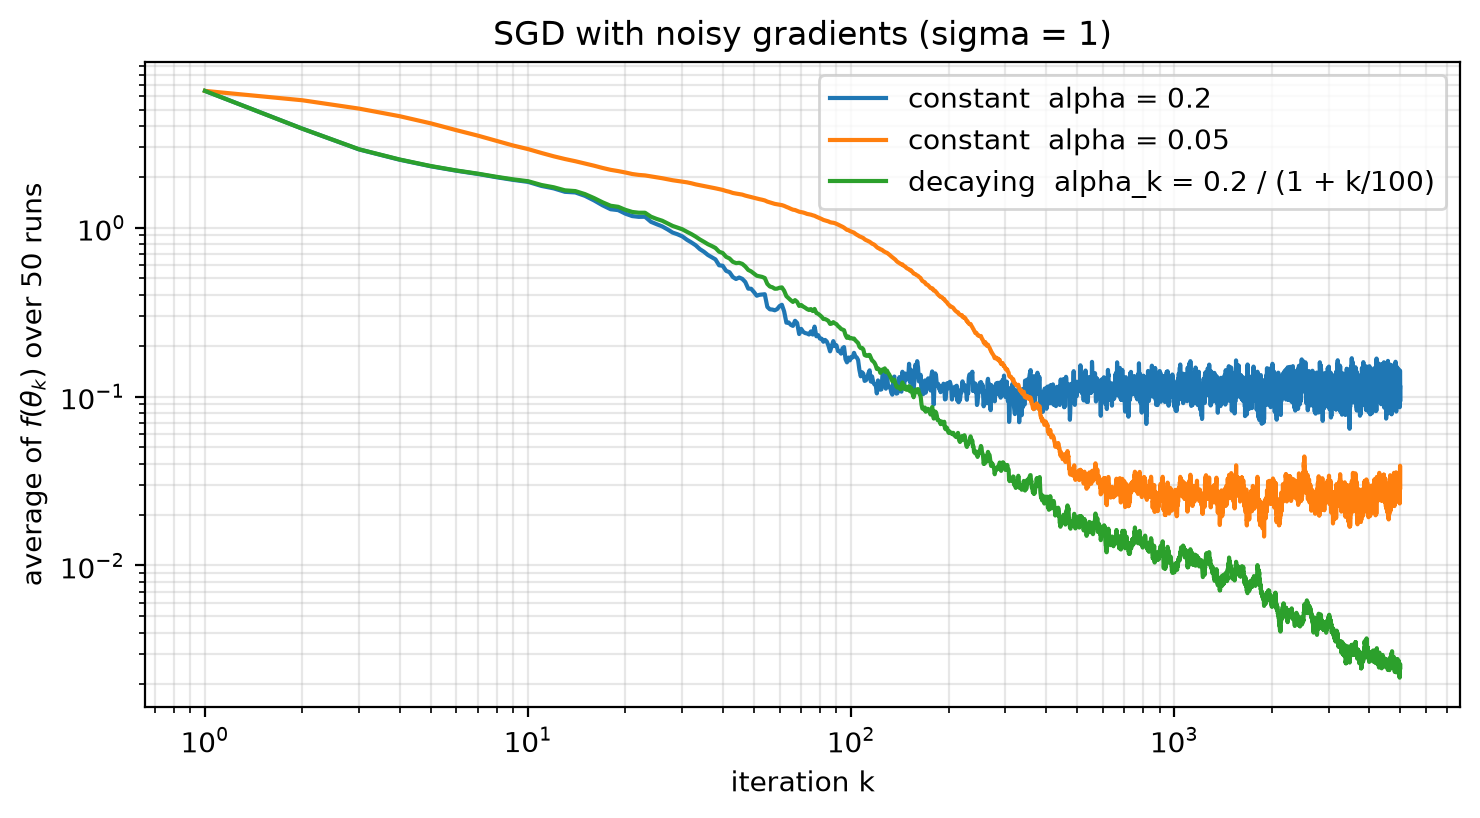
\includegraphics[width=0.78\textwidth]{figures/sgd_noise.png}

\small 잡음이 있는 gradient로 SGD를 했을 때 $f(\theta_k)$의 평균 ($50$번 반복, 로그-로그 눈금)
\end{center}
}{%
\begin{center}
\fbox{\parbox{0.8\textwidth}{\centering\small
[그림 자리] \texttt{figures/sgd\_noise.png}\\
\texttt{sgd\_noise\_2d.py}를 실행하면 생성된다.}}
\end{center}
}

\begin{center}
\begin{tabular}{@{}lcc@{}}
\toprule
학습률 & 이론값 $\lim\mathbb E[f]$ & 실험값 (마지막 $500$단계 평균) \\
\midrule
$\alpha=0.2$ (일정) & $0.113$ & $0.114$ \\
$\alpha=0.05$ (일정) & $0.026$ & $0.027$ \\
$\alpha_k=0.2/(1+k/100)$ (감소) & $0$으로 감소 & $0.0026$ (계속 감소 중) \\
\bottomrule
\end{tabular}
\end{center}

\paragraph{6. 학습률을 줄여 가면: Robbins--Monro 조건.}
잡음의 바닥을 없애려면 학습률을 점점 줄여야 한다. 얼마나 빨리 줄여야 할까?
Robbins와 Monro(1951)의 조건은
\[
\boxed{
\sum_{k=0}^{\infty}\alpha_k=\infty,
\qquad
\sum_{k=0}^{\infty}\alpha_k^2<\infty
}
\]
이다.
\begin{itemize}[leftmargin=1.8em]
\item $\sum\alpha_k=\infty$: 갈 수 있는 \textbf{총 거리}가 무한해야 한다.
학습률을 너무 빨리 줄이면 (예: $\alpha_k=\frac{1}{(k+1)^2}$, 합이 유한) 최솟값에 닿기 전에 멈춰 버릴 수 있다.
\item $\sum\alpha_k^2<\infty$: 3에서 잡음이 매 단계 더하는 양은 $\frac{M\alpha_k^2\sigma^2}{2}$이므로,
그 \textbf{총합이 유한}해야 잡음이 계속 쌓이지 않는다. 학습률이 일정하면 이 합이 무한이다.
\end{itemize}

\begin{center}
\begin{tabular}{@{}lccl@{}}
\toprule
학습률 $\alpha_k$ & $\sum\alpha_k$ & $\sum\alpha_k^2$ & 판정 \\
\midrule
$\alpha$ (일정) & $\infty$ & $\infty$ & 바닥에서 멈춤 \\
$\alpha_0/(1+k/k_0)$ ($\propto\frac1k$) & $\infty$ & 유한 & 조건 만족 \\
$\alpha_0/\sqrt{k+1}$ & $\infty$ & $\infty$ & 경계 (둘째 조건 불만족) \\
$\alpha_0/(k+1)^2$ & 유한 & 유한 & 너무 빨리 줄어듦 \\
\bottomrule
\end{tabular}
\end{center}

이 조건 아래에서 대표적으로 다음이 알려져 있다 (증명은 생략한다).
\begin{itemize}[leftmargin=1.8em]
\item 손실이 볼록(convex)하면 SGD는 최솟값으로 수렴한다.
\item 손실이 볼록하지 않으면 (신경망) gradient의 크기가 $0$으로 가는 점, 즉 \textbf{정류점(stationary point)}으로 수렴한다.
정류점은 극소점일 수도 있지만 안장점일 수도 있다.
\item 강볼록(strongly convex, 가장 작은 곡률이 $\mu>0$)인 경우 $\alpha_k\propto\frac1k$로 잡으면
$\mathbb E[L(\theta_k)]-L^*=O\!\left(\frac1k\right)$이다.
그림의 초록색 곡선이 로그-로그 눈금에서 기울기 약 $-1$인 직선처럼 내려가는 것이 이것이다.
잡음이 없는 경사하강법은 $(1-\alpha\mu)^k$처럼 \textbf{지수적으로} 빨리 줄어드는 것과 비교된다.
\end{itemize}

\paragraph{7. 실무와의 연결.}
\begin{itemize}[leftmargin=1.8em]
\item 실제 학습은 단계 수가 정해져 있으므로 Robbins--Monro 조건을 문자 그대로 따르지는 않지만,
\textbf{학습률 스케줄}(\ref{app:opt}.1절의 cosine 감소, 일정 epoch마다 $\frac1{10}$로 줄이는 step decay 등)은
모두 ``처음에는 크게 움직이고, 나중에는 잡음의 바닥을 낮추기 위해 학습률을 줄인다''는 같은 생각에서 나왔다.
\item 미니배치 크기 $h$를 키우면 $\sigma^2\propto\frac1h$가 작아져 바닥이 낮아진다.
학습률을 줄이는 것과 배치를 키우는 것이 비슷한 효과를 내는 이유이다.
\item 본문의 RMSProp 그림에서 최솟값 근처의 흔들림, 학생용 강의안의 MNIST 최적화 기법 비교 절의 MNIST 손실이 들쭉날쭉한 것도
같은 원리로 이해할 수 있다.
\item Adam 같은 적응적 방법도 이론적인 수렴 보장에는 주의가 필요하다.
볼록한 문제에서도 원래의 Adam이 수렴하지 않는 예가 알려져 있으며 (Reddi 등, 2018),
이를 고친 변형(AMSGrad 등)이 제안되었다. 실무에서는 대개 학습률 스케줄과 함께 사용한다.
\end{itemize}

% -------------------------------------------------
\subsection{Newton 방법을 그대로 쓸 수 없는 이유}
% -------------------------------------------------

``Gradient Descent와 Newton's method'' 시간에 본 Newton 방법은
\[
\theta_{k+1}=\theta_k-H_k^{-1}g_k
\]
였다. $H_k^{-1}$이 곡률이 큰 방향의 보폭은 줄이고 작은 방향의 보폭은 키워 주므로,
2차 함수에서는 \textbf{한 번에} 최솟값에 도달한다.
본문의 예제 $f(x,y)=\frac{1}{20}x^2+y^2$에서는 $H=\operatorname{diag}\bigl(\frac{1}{10},\,2\bigr)$이므로
\[
\theta_1=\begin{pmatrix}-7\\2\end{pmatrix}-\begin{pmatrix}10&0\\0&\tfrac12\end{pmatrix}\begin{pmatrix}-0.7\\4\end{pmatrix}
=\begin{pmatrix}0\\0\end{pmatrix}
\]
로 바로 최솟값이다. 그런데 신경망에서는 이것을 쓸 수 없다.

매개변수가 $n$개이면 $H$는 $n\times n$ 행렬이다.
\begin{itemize}[leftmargin=1.8em]
\item 지난주 MNIST의 작은 network만 해도 $n\approx8\times10^4$이므로 $H$의 원소는 약 $6.3\times10^9$개,
실수 하나에 8바이트이면 약 $50$GB이다.
\item 역행렬(또는 연립방정식 $Hp=-g$의 풀이)에는 $O(n^3)$의 계산이 든다.
\item 언어모델은 $n$이 수십억 이상이므로 아예 불가능하다.
\end{itemize}

\begin{center}
\begin{tabular}{@{}lll@{}}
\toprule
방법 & 메모리 & 한 단계의 계산량 \\
\midrule
SGD & $O(n)$ & $O(n)$ \\
모멘텀, Adam & $O(n)$ (상태 $1\sim2$개) & $O(n)$ \\
Newton & $O(n^2)$ & $O(n^3)$ \\
BFGS & $O(n^2)$ & $O(n^2)$ \\
L-BFGS & $O(mn)$ & $O(mn)$ \\
\bottomrule
\end{tabular}
\end{center}
(gradient 자체를 구하는 역전파의 비용은 모든 방법에 공통이므로 제외하였다. $m$은 L-BFGS가 기억하는 쌍의 개수.)

% -------------------------------------------------
\subsection{Quasi-Newton 방법: BFGS}
% -------------------------------------------------

\paragraph{아이디어: gradient의 변화로 곡률을 추정한다.}
Hessian을 직접 계산하지 않고, \textbf{이미 계산한 gradient들의 변화}로부터 곡률을 추정할 수 있다.
1변수라면
\[
f''(x_k)\approx\frac{f'(x_{k+1})-f'(x_k)}{x_{k+1}-x_k}
\]
인 것과 같은 생각이다.
연속한 두 단계에서
\[
s_k=\theta_{k+1}-\theta_k,
\qquad
y_k=g_{k+1}-g_k
\]
라 하면, 2차 함수 $L(\theta)=\frac12\theta\T A\theta$에서는 $g=A\theta$이므로 정확히 $y_k=As_k$이다.
일반적인 함수에서도 근사적으로
\[
\boxed{
H_{k+1}s_k\approx y_k
}
\qquad\text{(secant 조건)}
\]
가 성립한다.

\paragraph{BFGS의 갱신식.}
BFGS(Broyden--Fletcher--Goldfarb--Shanno)는 Hessian의 역행렬의 근사 $B_k\approx H_k^{-1}$을 직접 갱신한다.
새 근사 $B_{k+1}$이 secant 조건 $B_{k+1}y_k=s_k$를 만족하면서 $B_k$와 가장 가깝도록 정하면
\[
\boxed{
B_{k+1}=\bigl(I-\rho_k s_ky_k\T\bigr)\,B_k\,\bigl(I-\rho_k y_ks_k\T\bigr)+\rho_k s_ks_k\T,
\qquad
\rho_k=\frac{1}{y_k\T s_k}
}
\]
를 얻는다. 그리고 Newton 방향 대신
\[
p_k=-B_kg_k,
\qquad
\theta_{k+1}=\theta_k+t_k\,p_k
\]
로 움직인다. 이동 거리 $t_k$는 \textbf{line search}로 정한다.
\begin{itemize}[leftmargin=1.8em]
\item $y_k\T s_k>0$ (\textbf{곡률 조건})이면 $B_k$가 양의 정부호이면 $B_{k+1}$도 양의 정부호로 유지되어,
$p_k$가 항상 함수값이 줄어드는 방향($g_k\T p_k<0$)이 된다.
\item 2차 함수에서 정확한 line search를 쓰면 BFGS는 최대 $n$번 만에 최솟값에 도달한다.
\end{itemize}

\paragraph{Line search란?}
지금까지의 방법들은 학습률 $\alpha$라는 \textbf{정해진 보폭}으로 움직였다.
line search는 보폭을 미리 정하지 않는다.
먼저 갈 방향 $p_k$를 정한 뒤, 그 방향의 직선 $\theta_k+t\,p_k$ 위에서
\textbf{얼마나 갈지} $t$를 몇 번 시험해 보며 고른다.
예를 들어 $t=1$을 먼저 해 보고, 함수값이 충분히 줄지 않으면 $t$를 줄여서 다시 해 보는 식이다.
이때 확인하는 것은 두 가지이다.
\begin{itemize}[leftmargin=1.8em]
\item \textbf{너무 멀리 가지 않았는가}: 함수값이 충분히 줄었는가 (Armijo 조건)
\item \textbf{너무 덜 가지 않았는가}: 그 방향으로 아직 가파르게 내려가는 중은 아닌가 (곡률 조건)
\end{itemize}
좋은 보폭을 자동으로 찾아 주는 대신,
$t$를 하나 시험할 때마다 \textbf{함수값과 gradient를 다시 계산}해야 한다는 비용이 든다.

\paragraph{Line search: Wolfe 조건.}
수식으로는 $t_k$를 보통 다음 두 조건을 만족하는 값으로 정한다 ($0<c_1<c_2<1$, 예: $c_1=10^{-4}$, $c_2=0.9$).
\[
\begin{aligned}
&L(\theta_k+t\,p_k)\le L(\theta_k)+c_1\,t\,g_k\T p_k
&&\text{(충분히 감소: Armijo 조건)}\\
&\bigl|\nabla L(\theta_k+t\,p_k)\T p_k\bigr|\le c_2\,\bigl|g_k\T p_k\bigr|
&&\text{(기울기가 충분히 완만해짐: strong Wolfe 조건)}
\end{aligned}
\]
두 번째 조건이 곡률 조건 $y_k\T s_k>0$을 보장한다.
line search는 조건을 만족하는 $t$를 찾을 때까지 \textbf{함수값과 gradient를 여러 번 계산}한다는 점에 주목하자.

BFGS도 $B_k$라는 $n\times n$ 행렬을 저장해야 하므로 신경망에는 여전히 너무 크다.

% -------------------------------------------------
\subsection{L-BFGS: 최근 $m$개의 쌍만 기억한다}
% -------------------------------------------------

\textbf{L-BFGS}(Limited-memory BFGS)는 $B_k$를 저장하지 않는다.
대신 최근 $m$개(보통 $5\sim20$개)의 쌍 $(s_i,y_i)$만 기억하고,
BFGS 갱신식을 $m$번 적용했을 때의 $B_kg_k$를 다음 \textbf{two-loop recursion}으로 바로 계산한다.

\begin{remarkbox}[L-BFGS의 two-loop recursion: $r\approx B_kg_k$ 계산]
\begin{enumerate}[leftmargin=1.8em]
\item $q\leftarrow g_k$
\item $i=k-1,\ k-2,\ \ldots,\ k-m$에 대하여:\quad
$a_i\leftarrow\rho_i\,s_i\T q,\qquad q\leftarrow q-a_i\,y_i$
\item $r\leftarrow\gamma_k\,q$,\quad $\gamma_k=\dfrac{s_{k-1}\T y_{k-1}}{y_{k-1}\T y_{k-1}}$
\quad (처음 근사 $B_k^{(0)}=\gamma_kI$)
\item $i=k-m,\ \ldots,\ k-1$에 대하여:\quad
$b\leftarrow\rho_i\,y_i\T r,\qquad r\leftarrow r+s_i\,(a_i-b)$
\item 방향 $p_k=-r$
\end{enumerate}
벡터의 내적과 덧셈만 쓰므로 메모리와 계산량이 모두 $O(mn)$이다.
\end{remarkbox}

\paragraph{예제 함수에서의 L-BFGS.}
본문의 예제는 2차 함수이므로 Hessian이 상수이고, 앞에서 보았듯이 Newton 방법이면 \textbf{한 번}에 끝난다.
그런데도 L-BFGS를 적용해 보는 것은, 실제 신경망에서는 Newton 방법을 쓸 수 없고
실무에서 쓸 수 있는 2차 방법이 Hessian을 gradient의 변화로 근사하는 quasi-Newton 방법,
특히 L-BFGS이기 때문이다.
\textbf{Hessian을 한 번도 계산하지 않고도} 1차 방법보다 훨씬 빨리 수렴하는 모습을 확인해 보자.
PyTorch에는 \texttt{torch.optim.LBFGS}로 구현되어 있다.
L-BFGS는 line search 도중 함수값을 여러 번 다시 계산해야 하므로,
\textbf{손실을 다시 계산하는 함수(\texttt{closure})}를 \texttt{step}에 넘겨 준다.
이것이 다른 optimizer와 다른 점이다.

\begin{lstlisting}
import torch

w = torch.tensor([-7.0, 2.0], requires_grad=True)       # (x, y), start point

def f(w):
    return w[0] ** 2 / 20.0 + w[1] ** 2

# max_iter=1: one L-BFGS iteration per optimizer.step() (the default is 20)
optimizer = torch.optim.LBFGS([w], lr=1.0, max_iter=1, history_size=10,
                              line_search_fn="strong_wolfe")

n_eval = 0
def closure():                  # L-BFGS may evaluate f several times per step
    global n_eval
    n_eval += 1
    optimizer.zero_grad()
    loss = f(w)
    loss.backward()
    return loss

for k in range(1, 9):
    optimizer.step(closure)
    print(f"iteration {k}: (x, y) = ({w[0].item():9.6f}, {w[1].item():9.6f}),  "
          f"f = {f(w).item():.3e},  evaluations so far = {n_eval}")
\end{lstlisting}

\begin{center}
\begin{minipage}[c]{0.5\textwidth}
\centering
\begin{tabular}{@{}crrc@{}}
\toprule
반복 & \multicolumn{1}{c}{$x$} & \multicolumn{1}{c}{$y$} & $f$ \\
\midrule
1 & $-6.8511$ & $1.1489$ & $3.7\times10^{0}$ \\
2 & $-6.2977$ & $-0.0551$ & $2.0\times10^{0}$ \\
3 & $-5.9080$ & $-0.1358$ & $1.8\times10^{0}$ \\
4 & $-1.5216$ & $-0.3675$ & $2.5\times10^{-1}$ \\
5 & $-0.0928$ & $-0.0878$ & $8.1\times10^{-3}$ \\
6 & $0.0197$ & $-0.0050$ & $4.5\times10^{-5}$ \\
7 & $0.0024$ & $-0.0002$ & $3.1\times10^{-7}$ \\
8 & $0.0000$ & $0.0000$ & $9.3\times10^{-11}$ \\
\bottomrule
\end{tabular}
\end{minipage}%
\begin{minipage}[c]{0.48\textwidth}
\centering
\IfFileExists{figures/opt_lbfgs.png}{%
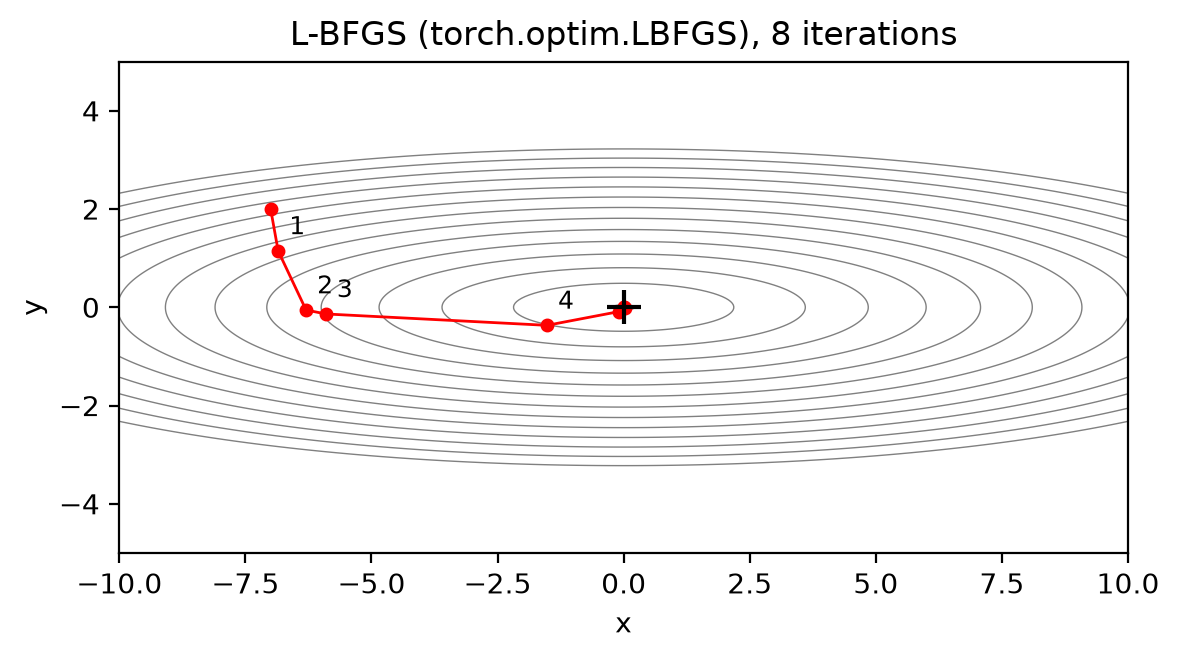
\includegraphics[width=\textwidth]{figures/opt_lbfgs.png}
}{%
\fbox{\parbox{0.9\textwidth}{\centering\small
[그림 자리] \texttt{figures/opt\_lbfgs.png}}}
}
\end{minipage}
\end{center}

\begin{itemize}[leftmargin=1.8em]
\item 첫 반복에서는 아직 쌍 $(s,y)$가 없으므로 gradient 방향으로 움직인다.
쌍이 쌓이면서 곡률을 반영한 방향으로 바뀌고, 4번째 반복부터 최솟값을 향해 크게 이동한다.
\item $8$번의 반복(함수값 계산 $16$번)만에 $f\approx10^{-10}$에 도달하였다.
본문에서 $30$번 갱신한 SGD, 모멘텀, AdaGrad, Adam은 $f\approx10^{-1}\sim10^{-3}$이었다.
\item 이론적으로 2차 함수에서는 $n=2$번 만에 끝나야 하지만,
PyTorch의 line search는 Wolfe 조건만 만족하면 멈추는 근사적인 방법이라 조금 더 걸린다.
\end{itemize}

% -------------------------------------------------
\subsection{L-BFGS가 딥러닝에서 잘 쓰이지 않는 이유}
% -------------------------------------------------

예제에서는 훨씬 빨랐는데, 왜 신경망 학습에는 Adam이나 SGD를 쓸까?

\paragraph{1. 미니배치 잡음.}
L-BFGS는 정확한 gradient를 가정한다.
그런데 미니배치 학습에서는 단계마다 다른 데이터 $\mathcal B_k$로 gradient를 계산한다.
미니배치 gradient를 $\nabla L_{\mathcal B}(\theta)=\nabla L(\theta)+\xi_{\mathcal B}$ (잡음 $\xi$)로 쓰면
\[
y_k=\nabla L_{\mathcal B_{k+1}}(\theta_{k+1})-\nabla L_{\mathcal B_k}(\theta_k)
=\underbrace{\nabla L(\theta_{k+1})-\nabla L(\theta_k)}_{\approx H s_k}
+\underbrace{\xi_{\mathcal B_{k+1}}-\xi_{\mathcal B_k}}_{\text{잡음}}
\]
이다. 보폭 $s_k$가 작아지면 첫 항은 $s_k$에 비례해 작아지지만 잡음 항은 줄지 않는다.
그래서 $y_k$와 $s_k$로 추정한 곡률이 \textbf{곡률이 아니라 데이터의 차이}를 반영하게 되어 근사가 무너진다
(곡률 조건 $y_k\T s_k>0$도 깨질 수 있다).
두 gradient를 같은 미니배치로 계산하는 변형들이 연구되었지만 널리 쓰이지는 않는다.

\paragraph{2. Line search의 비용.}
한 단계마다 함수값과 gradient를 여러 번 계산해야 한다.
큰 network에서 순전파와 역전파 한 번은 비싸므로,
그 계산으로 SGD나 Adam을 여러 걸음 가는 편이 대개 더 효율적이다.
게다가 미니배치 손실로 하는 line search 자체도 잡음 때문에 불안정하다.

\paragraph{3. 비볼록성.}
신경망의 손실함수는 볼록하지 않아 Hessian이 양의 정부호가 아닐 수 있다.
안장점(saddle point) 근처에서는 Hessian의 고유값이 음수인 방향이 있어서,
Newton 방향 $-H^{-1}g$가 오히려 함수값이 \textbf{올라가는} 방향일 수 있다.
quasi-Newton 방법은 곡률 조건을 만족하는 쌍만 쓰는 등의 장치로 이를 피하지만, 그만큼 곡률 정보가 부정확해진다.

\paragraph{4. 메모리.}
$m$개의 쌍만 저장해도 매개변수 전체를 $2m$번 복사해 두는 것과 같다.
$m=10$이면 매개변수의 $20$배이므로, 큰 모델에서는 상태를 $2$개만 가지는 Adam보다 훨씬 무겁다.

% -------------------------------------------------
\subsection{L-BFGS가 실제로 쓰이는 곳}
% -------------------------------------------------

반대로 위의 약점이 문제가 되지 않는 곳, 즉
\textbf{데이터 전체로 정확한 gradient를 계산할 수 있고, 높은 정밀도가 중요한} 문제에서는 L-BFGS가 매우 강력하다.

\begin{itemize}[leftmargin=1.8em]
\item \textbf{작은 문제의 full-batch 학습.}
scikit-learn의 로지스틱 회귀(\texttt{LogisticRegression})는 기본 solver가 \texttt{"lbfgs"}이다.
\item \textbf{PINN (Physics-Informed Neural Network).}
신경망 $u_\theta(x,t)$로 편미분방정식의 해를 근사하는 과학계산 방법이다.
예를 들어 방정식 $\mathcal N[u]=0$과 경계조건 $u=h$가 주어지면
\[
L(\theta)=\frac{1}{N_r}\sum_{i=1}^{N_r}\bigl|\mathcal N[u_\theta](x_i)\bigr|^2
+\frac{1}{N_b}\sum_{j=1}^{N_b}\bigl|u_\theta(x_j)-h(x_j)\bigr|^2
\]
을 최소화한다 (첫 항: 방정식의 잔차, 둘째 항: 경계조건).
점 $x_i$, $x_j$를 전체 배치로 쓸 수 있고 해의 정밀도가 중요하므로,
\textbf{Adam으로 먼저 대략 학습한 뒤 L-BFGS로 마무리}하는 방식이 표준처럼 쓰인다.
\item \textbf{신경 스타일 전이 (neural style transfer).}
network의 가중치가 아니라 \textbf{이미지 한 장}을 최적화하는 문제라 full-batch이므로 L-BFGS를 썼다 (Gatys 등).
\end{itemize}

\begin{thinkbox}[데이터 계산 과학과 L-BFGS]
수치해석과 과학계산에서는 L-BFGS가 오래전부터 표준적인 최적화 방법이었다.
딥러닝이 과학계산 문제(PINN, 역문제, 대리 모델 등)에 쓰이면서,
``미니배치 + Adam''과 ``full-batch + L-BFGS''를 상황에 맞게 함께 쓰는 일이 많아졌다.
어떤 경우에 어느 쪽이 유리한지는 위의 네 가지 이유로 판단할 수 있다.
\end{thinkbox}

% -------------------------------------------------
\subsection{대규모 딥러닝에서의 ``곡률 근사''}\label{app:largescale}
% -------------------------------------------------

Hessian을 통째로 다룰 수는 없지만, 곡률 정보를 \textbf{구조를 단순화하여} 근사하는 방법들이 있다.
모두 다음과 같은 \textbf{preconditioning}의 형태로 볼 수 있다.
\[
\boxed{
\theta_{k+1}=\theta_k-\alpha\,P_k^{-1}g_k
}
\]
\begin{center}
\begin{tabular}{@{}ll@{}}
\toprule
방법 & preconditioner $P_k$ \\
\midrule
SGD & $I$ \\
Newton & $H_k$ (전체 Hessian) \\
AdaGrad, RMSProp, Adam & $\operatorname{diag}(\sqrt{h_k})$ 또는 $\operatorname{diag}(\sqrt{\hat v_k})$ (대각 행렬) \\
K-FAC, Shampoo & 층마다 (작은 행렬) $\otimes$ (작은 행렬) 꼴 \\
\bottomrule
\end{tabular}
\end{center}

\paragraph{Adam은 대각 근사이다.}
Adam이 $\sqrt{\hat v}$로 나누는 것은 매개변수마다(대각 성분마다) 보폭을 조절하는 것이다.
$\hat v$는 Hessian 자체는 아니지만 gradient 제곱의 평균으로 곡률의 크기를 대신하는 역할을 하며,
본문에서 ``AdaGrad가 Newton의 곡률 보정과 비슷한 효과''라고 한 것이 이 뜻이다.
그러나 대각 행렬은 매개변수 \textbf{사이의} 관계(Hessian의 비대각 성분)를 반영하지 못한다.

\paragraph{Hessian-free 방법.}
Newton 방향은 연립방정식 $H_kp=-g_k$의 해이다.
$H_k$를 만들지 않고도 \textbf{Hessian과 벡터의 곱} $H_kv$는
\[
H_kv=\nabla_\theta\bigl(\nabla_\theta L(\theta)\T v\bigr)
\]
로, 역전파를 한 번 더 하는 정도의 비용으로 계산할 수 있다.
켤레기울기법(conjugate gradient)은 행렬 대신 이 곱만 사용하여 $H_kp=-g_k$를 근사적으로 푸므로,
$H_k$를 저장하지 않고 Newton 방향을 근사할 수 있다 (Martens, 2010).

\paragraph{K-FAC.}
한 affine 계층 $A=XW$ ($X$: $h\times l$, $W$: $l\times m$)에서
지난주에 $\pd{L}{W}=X\T\delta$ ($\delta=\pd{L}{A}$, $h\times m$)를 얻었다.
K-FAC은 이 층의 곡률 행렬(정확히는 Fisher 정보 행렬)을 입력 쪽 통계
$\bar A=\frac1h X\T X$ ($l\times l$)와 출력 쪽 통계 $\bar G=\frac1h\delta\T\delta$ ($m\times m$)의
\textbf{크로네커 곱}으로 근사한다. 그러면 $(lm)\times(lm)$ 행렬 대신 작은 두 행렬의 역행렬만 있으면 되고,
갱신 방향은
\[
\Delta W=-\alpha\,\bar A^{-1}\,\pd{L}{W}\,\bar G^{-1}
\]
꼴이 된다 (실제로는 역행렬이 잘 정의되도록 작은 값을 더한다).

\paragraph{Shampoo.}
층의 gradient 행렬 $G_k=\pd{L}{W}$ ($l\times m$)에 대해 양쪽 통계를 누적하여
\[
L_k=\sum_{j\le k}G_jG_j\T\ (l\times l),
\qquad
R_k=\sum_{j\le k}G_j\T G_j\ (m\times m),
\qquad
W_{k+1}=W_k-\alpha\,L_k^{-1/4}\,G_k\,R_k^{-1/4}
\]
로 갱신한다. 매개변수가 하나뿐이면 $L_k=R_k=\sum g_j^2$이므로 $G_k/\sqrt{\sum g_j^2}$,
즉 AdaGrad와 같아진다. Shampoo는 \textbf{AdaGrad를 행렬로 확장}한 방법이다.

\paragraph{Muon.}
층의 gradient로 모멘텀 $M_k=\beta M_{k-1}+G_k$를 만든 뒤,
$M_k$의 특이값 분해 $M_k=U\Sigma V\T$에서 특이값을 모두 $1$로 바꾼 행렬 $UV\T$
(가장 가까운 직교 행렬)의 방향으로 갱신한다.
\[
W_{k+1}=W_k-\alpha\,\operatorname{orth}(M_k),
\qquad
\operatorname{orth}(M)=UV\T
\]
특이값 분해는 비싸므로 실제로는 행렬곱만 쓰는 Newton--Schulz 반복으로 $UV\T$를 근사한다.
모든 방향의 크기를 고르게 맞춘다는 점에서 역시 곡률 보정의 한 형태로 볼 수 있다.
Shampoo와 Muon은 최근 대규모 모델 학습에서 실제로 쓰이기 시작했지만,
아직 AdamW만큼 표준은 아니다.

\begin{keybox}[부록 정리]
\begin{itemize}[leftmargin=1.5em]
\item 요즘 실무의 기본은 \textbf{AdamW}, 이미지 분류 CNN에서는 \textbf{SGD + 모멘텀}이다.
AdaGrad는 RMSProp, Adam으로 이어지는 아이디어의 출발점으로 배운다.
\item optimizer만큼, 때로는 그보다 \textbf{학습률 스케줄}과 weight decay가 중요하다.
\item 잡음이 있는 gradient로 학습률을 고정하면 SGD는 $\alpha\sigma^2$에 비례하는 \textbf{잡음의 바닥}에서 멈춘다.
$\sum\alpha_k=\infty$, $\sum\alpha_k^2<\infty$ (Robbins--Monro)를 만족하도록 학습률을 줄이면 수렴한다.
\item Newton 방법은 $O(n^2)$ 메모리, $O(n^3)$ 계산 때문에 신경망에 쓸 수 없다.
\item L-BFGS는 gradient의 변화로 곡률을 근사하여 $O(mn)$로 줄인다.
full-batch로 정밀하게 풀어야 하는 문제(PINN, 작은 모델)에서는 강력하지만,
미니배치 잡음, line search 비용, 비볼록성, 메모리 때문에 대규모 딥러닝에서는 잘 쓰이지 않는다.
\item 대규모 딥러닝의 곡률 활용은 \textbf{구조를 단순화한 preconditioner}로 이루어진다:
Adam(대각), K-FAC과 Shampoo(층별 크로네커 곱), Muon(직교화).
\end{itemize}
\end{keybox}


\end{document}
